\documentclass[12pt,border=4pt,multi]{article}%\documentclass[tikz,border=4pt,multi]{article}
\usepackage{lingmacros}
\usepackage{tree-dvips}
\usepackage{amssymb} %for mathbb{}
\usepackage[dvipsnames]{xcolor}
\usepackage{forest}
\usepackage{amsmath} %for matrices
\usepackage{xeCJK}
\usepackage{tikz}
\usepackage[arrowdel]{physics}
\usepackage{graphicx}
\usepackage{wrapfig}
\usepackage{listings}
\graphicspath{{./img}} %specify the graphics path to be relative to the main .tex file, denoting the main .tex file directory as ./
\usepackage{esint}
\newcommand\Myperm[2][^n]{\prescript{#1\mkern-2.5mu}{}P_{#2}}
\newcommand\Mycomb[2][^n]{\prescript{#1\mkern-0.5mu}{}C_{#2}}
\definecolor{orchid}{rgb}{0.7, 0.4, 1.1}

\begin{document}

\section*{Xi Liu, xl3504, Homework 2}
Problem 1\\
(a)\\
reverse pairs of array [2, 3, 8, 6, 1]:\\
(1, 5), (2, 5), (3, 4), (3, 5), (4, 5)\\
\\
\\
\\
\\
\\
(b)\\
claim:\\
when the array is sorted in descending order, the running time of INSERTION\_SORT is $\Theta(n^2)$, the number of reverse pairs is maximized: largest number of reverse pairs = $n(n - 1) / 2$\\
when the array is sorted in ascending order, the running time of INSERTION\_SORT is $\Theta(n)$, the number of reverse pairs is minimized: smallest number of reverse pairs = 0\\
\\
justification:\\
let array $A = [a_1,\; a_2,\; ...,\; a_n]$, let $a_i$ represent the element $A[i],\;\;\forall i \in [1, n] \cap \mathbb{N}$\\
\\
largest number of reverse pairs happen when array is sorted in descending order: $a_1 \geq a_2 \geq ... \geq a_n$, there will be $n - i$ reverse pairs containing the $i$th index, then
\[\text{largest number of reverse pairs} = (n - 1) + (n - 2) + ... + 1\]
\[= \sum_{i = 1}^{n - 1} (n - i) = \sum_{i = 1}^{n - 1} i = \frac{(n - 1)((n - 1) + 1)}{2} = \frac{n(n - 1)}{2}\]
\\
\\
smallest number of reverse pairs happen when array is sorted in ascending order: $a_1 \leq a_2 \leq ... \leq a_n$, smallest number of reverse pairs = 0\\
\\
\\
\\
\\
\begin{table}[htb]
    \begin{tabular}{llll} %left align
    & INSERTION\_SORT(A) & cost & times\\ 
    1 & \textbf{for} $j = 2$ to $A.length$ & $c_1$ & $n$\\
    2 & \quad $key = A[j]$ & $c_2$ & $n - 1$\\
    3 & \quad //insert $A[j]$ into the sorted\\
      & \quad \; sequence $A[1...j - 1]$ & $0$ & $n - 1$\\
    4 & \quad $i = j - 1$ & $c_4$ & $n - 1$\\
    5 & \quad \textbf{while} $i > 0$ and $A[i] > key$ & $c_5$ & $\sum_{j=2}^{n} t_j$\\
    6 &  \qquad\; $A[i + 1] = A[i]$ & $c_6$ & $\sum_{j=2}^{n} (t_j - 1)$\\
    7 &  \qquad\; $i = i - 1$ & $c_7$ & $\sum_{j=2}^{n} (t_j - 1)$\\
    8 &  \quad $A[i + 1] = key$ & $c_8$ & $n - 1$\\
    \end{tabular}
\end{table}
\[T(n) = \sum (cost)\cdot(times)\]
\[\textbf{equation 1:}\]
\[
T(n) = c_1 n + c_2 (n - 1) + c_4 (n - 1) + c_5 \sum_{j=2}^{n} t_j + c_6 \sum_{j=2}^{n} (t_j - 1) + c_7 \sum_{j=2}^{n} (t_j - 1) + c_8 (n - 1)
\]
worst case: if array is in reverse sorted order (decreasing order),\\
must compare each element $key = A[j]$ with each element in the entire sorted subarray $A[1...j - 1]$, so $t_j = j$ for $j = 2, 3, ..., n$\\ 
substitute $j$ for $t_j$ into equation 1, worst case running time is
\[T(n) = c_1 n + c_2 (n - 1) + c_4 (n - 1) + c_5 \sum_{j=2}^{n} j + c_6 \sum_{j=2}^{n} (j - 1) + c_7 \sum_{j=2}^{n} (j - 1) + c_8 (n - 1)\]
\[T(n) = c_1 n + c_2 (n - 1) + c_4 (n - 1) + c_5 \left( \frac{n(n + 1)}{2} - 1 \right) \]
\[+ c_6 \left( \frac{n(n - 1)}{2} \right) + c_7 \left( \frac{n(n - 1)}{2} \right) + c_8 (n - 1)\]
\begin{align*}
&= \left( \frac{c_5}{2} + \frac{c_6}{2} + \frac{c_7}{2}\right) n^2 + \left(c_1 + c_2 + c_4 + \frac{c_5}{2} - \frac{c_6}{2} - \frac{c_7}{2} + c_8\right) n
- (c_2 + c_4 + c_5 + c_8)\\
&= \Theta(n^2)\\
\end{align*}
\\
\\
\\
\\
insertion sort's best case is when the array is sorted in ascending order, then $A[i] \leqslant key$ for line 5, thus $t_j = 1$ for $j = 2,3,...,n$\\ 
substitute $1$ for $t_j$ into equation 1, best case running time is
\begin{align*}
    T(n) &= c_1 n + c_2 (n - 1) + c_4 (n - 1) + c_5(n - 1) + c_8 (n - 1)\\
    &= (c_1 + c_2 + c_4 + c_5 + c_8)n - (c_2 + c_4 + c_5 + c_8)\\
    &= \Theta(n)\\
\end{align*}
\\
\\
\\
\\
(c)\\
/* count\_reverse\_pairs() is an algorithm that determines the number of reverse pairs in an array of n numbers in $\Theta(n \lg n)$ run time */
\begin{lstlisting}[mathescape = true, escapeinside={;*}{*;)}, language = c]
int merge(int A[], int p, int q, int r)
{
    int left_len = q - p + 1; 
    int right_len = r - q;
    int L[left_len + 1];
    int R[right_len + 1];
    L[left_len + 1] = $\infty$;
    R[right_len + 1] = $\infty$;
    for(int i = 1; i < left_len; i++)
        L[i] = A[p + i];
    for(int i = 1; i < right_len; i++)
        R[i] = A[(q + 1) + i];
    int i = 1;
    int j = 1;
    int counter = 0;
    for(int k = p; k < r; k++)
    {
        if(L[i] <= right[r_i])
        {
            A[k] = L[i];
            i = i + 1;
        }
        else
        {
            A[k] = R[j];
            j = j + 1;
            counter = counter + left_len - i + 1;
        }
    }
    return counter;
}

int count_reverse_pairs(int A[], int p, int r)
{
    int c = 0;
    if(p < r)
    {
        int q = p + $\lfloor$ (r - p) / 2 $\rfloor$;
        int left = count_reverse_pairs(A, p, q);
        int right = count_reverse_pairs(A, q + 1, r);
        c = left + right + merge(A, p, q, r);
    }
    return c;
}
\end{lstlisting}
\newpage
\noindent
correctness of merge\\
\textbf{loop invariant:}\\
at the start of the each for iteration (the loop that rewrites original array $A$ using elements in $L$ and $R$ arrays), $A[p...k - 1]$ contains $final\_index - initial\_index + 1 = (k - 1) - p + 1 = k - p$ smallest elements of $L$ and $R$, in sorted order, $counter$ stores the number of reverse pairs $(a,\;b)$ such that $p \leq a < p + i - 1$ and $q + 1 \leq b \leq j$\\
Moreover, $L[i]$ and $R[j]$ are smallest elements of their arrays that have not been copied back to $A$\\
\\
\textbf{initialization}:\\ 
before first iteration of the loop, $k = p = 1$, so subarray $A[p...k - 1]$ is empty. This empty subarray contains $k - p = 0$ smallest elements of $L$ and $R$. Since $i = j = 1$, both $L[i]$ and $R[j]$ are the smallest elements of their arrays that have not been copied back to $A$, $i = 1$, $p \leq a < p + 1 - 1$, since $a \geq p$ and $a < p$ is a contradiction, there is no such number $a$ so there are no reverse pairs and $counter$ is 0\\
\\
\textbf{maintenance}: $P(k) \rightarrow P(k + 1)$\\
if $L[i] > R[j]$, then $R[j]$ is the smallest element that has not yet copied back into $A$,\\
based on the inductive hypothesis (loop invariant), $A[p...k - 1]$ contains $k - p$ smallest elements of array $L$ and $R$, and $counter$ stores the number of reverse pairs $(a,\;b)$ such that $p \leq a < p + i - 1$ and $q + 1 \leq b \leq j$
$\;\;(P(k))$.\\
after $L[i]$ is copied into $A[k]$, the subarray $A[p...k]$ contains $final\_index - initial\_index + 1 = k - p + 1$ smallest elements of array $L$ and $R$. since the assumption is $L[i] > R[j]$, so $R[j]$ is less than left\_len - i + 1 elements of $L[i...left\_len]$, but $i < j$, so there are left\_len - i + 1 reverse pairs associated with $L[i...left\_len]$ and $R[j]$, so after adding left\_len - i + 1 to $counter$ and increment $j$ by 1 and increment $k$ by 1, the loop invariant is maintained for $k + 1$ $\;\;(P(k + 1))$.\\
if $L[i] \leq R[j]$, then merge appropriate action to maintain the loop invariant with the roles of $L$ and $R$ interchanged\\
\\
\textbf{termination}:\\
at termination, $k = r + 1$, $i = \;$left\_len, $j = \;$right\_len. By the loop invariant, the subarray $A[p...k - 1] = A[p...(r + 1) - 1] = A[p...r]$, contains $final\_index - initial\_index + 1 = r - p + 1$ smallest elements of $L[1...n_1 + 1]$ and $R[1...n_2 + 1]$ in sorted order, $counter$ completed the addition of all reverse pairs $(a,\;b)$ associated with $L[i...$left\_len] and $R[j]$ for all $p \leq i \leq p \; + \;$left\_len, $q + 1 \leq j \leq q\; + \; $right\_len, $p \leq a < p + i - 1$, and $q + 1 \leq b \leq j$\\
\\
\\
\\
show $\Theta(n\lg n)$ is the run time bounds of count\_reverse\_pairs():\\
recurrence is given by\\
$T(n) =
\begin{cases}
    \Theta(1) & if\;n = 1\\
    T(\lceil n / 2 \rceil) + T(\lfloor n / 2 \rfloor) + \Theta(n) & if\;n > 1\\
\end{cases}
$\\
\\
assume $T(n) \leq c(n - 2)\lg(n - 2)$ is true for all positive $m < n$, in particular for $m = \lceil n / 2 \rceil$ and $m = \lfloor n / 2 \rfloor$, or equivalently assume $T(\lceil n / 2 \rceil) \leq c(\lceil n / 2 \rceil - 2)\lg(\lceil n / 2 \rceil - 2)$ and $T(\lfloor n / 2 \rfloor) \leq c(\lfloor n / 2 \rfloor - 2)\lg(\lfloor n / 2 \rfloor - 2)$\\
assume $\Theta(n) = kn$ for the recurrence stated above, where $k$ is a positive constant\\
\begin{align*}
    T(n) &= \textcolor{orchid}{T(\lceil n / 2 \rceil)} + \textcolor{orchid}{T(\lfloor n / 2 \rfloor)} + kn\\
    &\leq \textcolor{orchid}{c(\lceil n / 2 \rceil - 2)\lg(\lceil n / 2 \rceil - 2)} + \textcolor{orchid}{c(\lfloor n / 2 \rfloor - 2)\lg(\lfloor n / 2 \rfloor - 2)} + kn\\
    &\leq c(n / 2 + 1 - 2)\lg(n / 2 + 1 - 2) + c(n / 2 + 1 - 2)\lg(n / 2 + 1 - 2) + kn\\
    &= 2c(n / 2 + 1 - 2)\lg(n / 2 + 1 - 2) + kn\\
    &= 2c(n / 2 - 1)\lg(n / 2 - 1) + kn\\
    &= 2c((n - 2)/ 2)\lg((n - 2)/ 2) + kn\\
    &= c(n - 2)\lg((n - 2)/ 2) + kn\\
    &= c(n - 2)(\lg(n - 2) - \lg 2) + kn\\
    &= c(n - 2)(\lg(n - 2) - 1) + kn\\
    &= c(n - 2)\lg(n - 2) - c(n - 2) + kn\\
    &= c(n - 2)\lg(n - 2) + n(k - c) + 2c\\
    &= c(n - 2)\lg(n - 2) - (n(c - k) - 2c)\\
    &\leq c(n - 2)\lg(n - 2) \qquad if\;n(c - k) - 2c \geq 0\\
\end{align*}
\[n(c - k) - 2c \geq 0\]
\[n(c - k) \geq 2c\]
\[n \geq \frac{2c}{c - k}\]
\[\text{pick} \quad n \geq n_0 = \frac{2c}{c - k} \quad \text{and} \quad c > k\]
so
\[T(n) = O(n \lg n)\]
\\
\\
\\
\\
need to show $T(n) \geq cn\lg n$ for all $n \geq n_0$, where $c$ and $n_0$ are positive constants\\
\\
assume $T(n) \geq c(n + 2)\lg(n + 2)$ is true for all positive $m < n$, in particular for $m = \lceil n / 2 \rceil$ and $m = \lfloor n / 2 \rfloor$, or equivalently assume $T(\lceil n / 2 \rceil) \geq c(\lceil n / 2 \rceil + 2)\lg(\lceil n / 2 \rceil + 2)$ and $T(\lfloor n / 2 \rfloor) \geq c(\lfloor n / 2 \rfloor + 2)\lg(\lfloor n / 2 \rfloor + 2)$
\begin{align*}
    T(n) &= \textcolor{orchid}{T(\lceil n / 2 \rceil)} + \textcolor{orchid}{T(\lfloor n / 2 \rfloor)} + kn\\
    &\geq c(\lceil n / 2 \rceil + 2)\lg(\lceil n / 2 \rceil + 2) + c(\lfloor n / 2 \rfloor + 2)\lg(\lfloor n / 2 \rfloor + 2) + kn\\
    &\geq c(n / 2 - 1 + 2)\lg(n / 2 - 1 + 2) + c(n / 2 - 1 + 2)\lg(n / 2 - 1 + 2) + kn\\
    &\geq 2c(n / 2 - 1 + 2)\lg(n / 2 - 1 + 2) + kn\\
    &= 2c(n / 2 + 1)\lg(n / 2 + 1) + kn\\
    &= 2c((n + 2) / 2)\lg((n + 2) / 2) + kn\\
    &= c(n + 2)(\lg(n + 2) - \lg 2) + kn\\
    &= c(n + 2)\lg(n + 2) - c(n + 2) + kn\\
    &= c(n + 2)\lg(n + 2) + n(k - c) - 2c\\
    &\geq c(n + 2)\lg(n + 2)\\
    &if\;n(k - c) - 2c \geq 0, \quad
    i.e. \quad n \geq \frac{2c}{k - c}\\
\end{align*}
\[\text{pick} \quad n \geq n_0 = \frac{2c}{k - c} \quad \text{and} \quad k > c\]
so 
\[T(n) = \Omega(n \lg n)\]
since $T(n) = O(n \lg n)$ and $T(n) = \Omega(n \lg n)$, so $T(n) = \Theta(n \lg n)$
\newpage
\noindent
Problem 2\\
(a)\\
$T(n) =
\begin{cases}
    \Theta(1) & if\;n = 1\\
    4T(n / 4) + \Theta(n) & if\;n > 1\\
\end{cases}
$\\
\\
\\
\\
(b)
\\
\\
\\
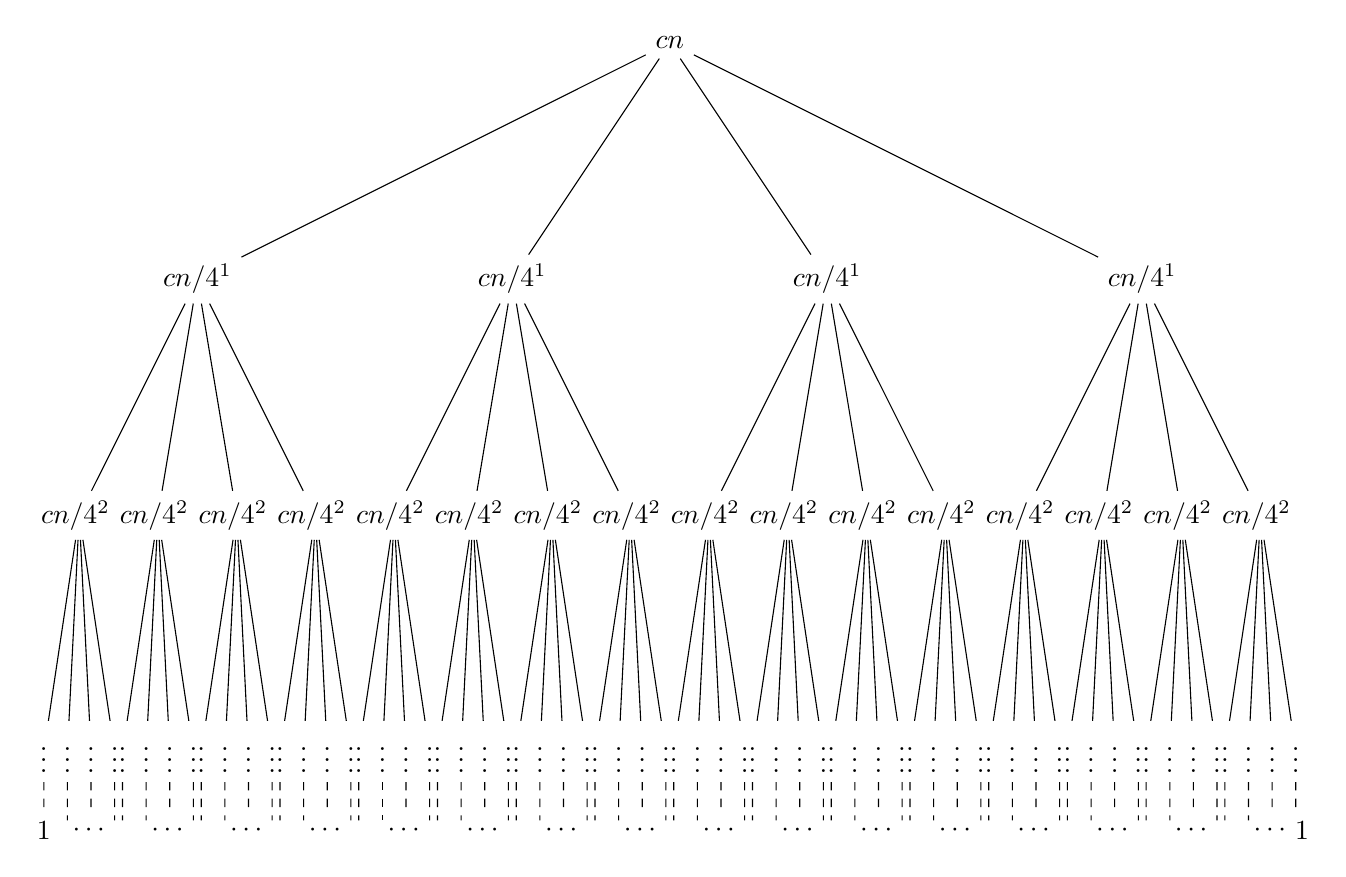
\begin{tikzpicture}
[
    level 1/.style = {sibling distance = 4cm, level distance = 3cm},
    level 2/.style = {sibling distance = 1cm, level distance = 3cm},
    level 3/.style = {sibling distance = 0.3cm, level distance = 3cm},
    level 4/.style = {sibling distance = 0.3cm, level distance = 1cm},
]
\node {$cn$}
    child{node{$cn / 4^1$}
        child{node{$cn / 4^2\;$}
            child{node{$\vdots$}
                child{node{1}
                edge from parent [dashed]}
            }
            child{node{$\vdots$}
                child{node{}
                edge from parent [dashed]}
            }
            child{node{$\vdots$}
                child{node{$\cdots$}
                edge from parent [dashed]}
            }
            child{node{$\vdots$}
                child{node{}
                edge from parent [dashed]}
            }
        }
        child{node{$cn / 4^2\;$}
            child{node{$\vdots$}
                child{node{}
                edge from parent [dashed]}
            }
            child{node{$\vdots$}
                child{node{}
                edge from parent [dashed]}
            }
            child{node{$\vdots$}
                child{node{$\cdots$}
                edge from parent [dashed]}
            }
            child{node{$\vdots$}
                child{node{}
                edge from parent [dashed]}
            }
        }
        child{node{$cn / 4^2\;$}
            child{node{$\vdots$}
                child{node{}
                edge from parent [dashed]}
            }
            child{node{$\vdots$}
                child{node{}
                edge from parent [dashed]}
            }
            child{node{$\vdots$}
                child{node{$\cdots$}
                edge from parent [dashed]}
            }
            child{node{$\vdots$}
                child{node{}
                edge from parent [dashed]}
            }
        }
        child{node{$cn / 4^2\;$}
            child{node{$\vdots$}
                child{node{}
                edge from parent [dashed]}
            }
            child{node{$\vdots$}
                child{node{}
                edge from parent [dashed]}
            }
            child{node{$\vdots$}
                child{node{$\cdots$}
                edge from parent [dashed]}
            }
            child{node{$\vdots$}
                child{node{}
                edge from parent [dashed]}
            }
        }
    }
    child {node {$cn / 4^1$}
        child{node{$cn / 4^2\;$}
            child{node{$\vdots$}
                child{node{}
                edge from parent [dashed]}
            }
            child{node{$\vdots$}
                child{node{}
                edge from parent [dashed]}
            }
            child{node{$\vdots$}
                child{node{$\cdots$}
                edge from parent [dashed]}
            }
            child{node{$\vdots$}
                child{node{}
                edge from parent [dashed]}
            }
        }
        child{node{$cn / 4^2\;$}
            child{node{$\vdots$}
                child{node{}
                edge from parent [dashed]}
            }
            child{node{$\vdots$}
                child{node{}
                edge from parent [dashed]}
            }
            child{node{$\vdots$}
                child{node{$\cdots$}
                edge from parent [dashed]}
            }
            child{node{$\vdots$}
                child{node{}
                edge from parent [dashed]}
            }
        }
        child{node{$cn / 4^2\;$}
            child{node{$\vdots$}
                child{node{}
                edge from parent [dashed]}
            }
            child{node{$\vdots$}
                child{node{}
                edge from parent [dashed]}
            }
            child{node{$\vdots$}
                child{node{$\cdots$}
                edge from parent [dashed]}
            }
            child{node{$\vdots$}
                child{node{}
                edge from parent [dashed]}
            }
        }
        child{node{$cn / 4^2\;$}
            child{node{$\vdots$}
                child{node{}
                edge from parent [dashed]}
            }
            child{node{$\vdots$}
                child{node{}
                edge from parent [dashed]}
            }
            child{node{$\vdots$}
                child{node{$\cdots$}
                edge from parent [dashed]}
            }
            child{node{$\vdots$}
                child{node{}
                edge from parent [dashed]}
            }
        }
    }
    child {node {$cn / 4^1$}
        child{node{$cn / 4^2\;$}
            child{node{$\vdots$}
                child{node{}
                edge from parent [dashed]}
            }
            child{node{$\vdots$}
                child{node{}
                edge from parent [dashed]}
            }
            child{node{$\vdots$}
                child{node{$\cdots$}
                edge from parent [dashed]}
            }
            child{node{$\vdots$}
                child{node{}
                edge from parent [dashed]}
            }
        }
        child{node{$cn / 4^2\;$}
            child{node{$\vdots$}
                child{node{}
                edge from parent [dashed]}
            }
            child{node{$\vdots$}
                child{node{}
                edge from parent [dashed]}
            }
            child{node{$\vdots$}
                child{node{$\cdots$}
                edge from parent [dashed]}
            }
            child{node{$\vdots$}
                child{node{}
                edge from parent [dashed]}
            }
        }
        child{node{$cn / 4^2\;$}
            child{node{$\vdots$}
                child{node{}
                edge from parent [dashed]}
            }
            child{node{$\vdots$}
                child{node{}
                edge from parent [dashed]}
            }
            child{node{$\vdots$}
                child{node{$\cdots$}
                edge from parent [dashed]}
            }
            child{node{$\vdots$}
                child{node{}
                edge from parent [dashed]}
            }
        }
        child{node{$cn / 4^2\;$}
            child{node{$\vdots$}
                child{node{}
                edge from parent [dashed]}
            }
            child{node{$\vdots$}
                child{node{}
                edge from parent [dashed]}
            }
            child{node{$\vdots$}
                child{node{$\cdots$}
                edge from parent [dashed]}
            }
            child{node{$\vdots$}
                child{node{}
                edge from parent [dashed]}
            }
        }
    }
    child {node {$cn / 4^1$}
        child{node{$cn / 4^2\;$}
            child{node{$\vdots$}
                child{node{}
                edge from parent [dashed]}
            }
            child{node{$\vdots$}
                child{node{}
                edge from parent [dashed]}
            }
            child{node{$\vdots$}
                child{node{$\cdots$}
                edge from parent [dashed]}
            }
            child{node{$\vdots$}
                child{node{}
                edge from parent [dashed]}
            }
        }
        child{node{$cn / 4^2\;$}
            child{node{$\vdots$}
                child{node{}
                edge from parent [dashed]}
            }
            child{node{$\vdots$}
                child{node{}
                edge from parent [dashed]}
            }
            child{node{$\vdots$}
                child{node{$\cdots$}
                edge from parent [dashed]}
            }
            child{node{$\vdots$}
                child{node{}
                edge from parent [dashed]}
            }
        }
        child{node{$cn / 4^2\;$}
            child{node{$\vdots$}
                child{node{}
                edge from parent [dashed]}
            }
            child{node{$\vdots$}
                child{node{}
                edge from parent [dashed]}
            }
            child{node{$\vdots$}
                child{node{$\cdots$}
                edge from parent [dashed]}
            }
            child{node{$\vdots$}
                child{node{}
                edge from parent [dashed]}
            }
        }
        child{node{$cn / 4^2\;$}
            child{node{$\vdots$}
                child{node{}
                edge from parent [dashed]}
            }
            child{node{$\vdots$}
                child{node{}
                edge from parent [dashed]}
            }
            child{node{$\vdots$}
                child{node{$\cdots$}
                edge from parent [dashed]}
            }
            child{node{$\vdots$}
                child{node{\;\,1}
                edge from parent [dashed]}
            }
        }
    };
\end{tikzpicture}
at depth $i$, number of nodes $= 4^i$\\
for a node at at depth $i$, subproblem size = $n / 4^i$\\
subproblem size = 1 = $n/4^i  \quad \rightarrow \quad 4^i = n \quad \rightarrow \quad \log_4 n = i$\\
so the tree have $\log_4 n + 1$ levels\\
number of leaves = $4^{\log_4 n} = n$\\
\\
time complexity at depth $i$ = (number of nodes at depth $i$)(cost of 1 node) = $(4^i)(cn / 4^i) = cn$\\
\begin{align*}
T(n) &= \sum_{i = 0}^{\log_4 n - 1} cn + \Theta(n)\\
&= (\log_4 n - 1 + 1)(cn) + \Theta(n)\\
&= cn\log_4 n + \Theta(n)\\
&= \Theta(n \lg n)
\end{align*}
\\
\\
\\
\\
(c)\\
show $\Theta(n\lg n)$ is the run time bounds of the variant of MERGE\_SORT that splits the array into four parts of almost equal sizes:\\
\\
base step is when $n = 4$, then $T(n) = T(4) = 4T(4 / 4) + \Theta(4) = 4T(1) + \Theta(4) = 4 + \Theta(4) = \Theta(1) \leq c(4)\lg 4 = 4c$\\
assume $T(n) \leq cn\lg n$ is true for all positive $m < n$, in particular for $m = n / 4$, or equivalently assume $T(n / 4) \leq c(n / 4)\lg(n / 4)$\\
assume $\Theta(n) = kn$ for the recurrence stated above, where $k$ is a positive constant\\
\begin{align*}
    T(n) &= 4\textcolor{orchid}{T(n / 4)} + kn\\
    &\leq 4\textcolor{orchid}{c(n / 4)\lg(n / 4)} + kn\\
    &= cn\lg(n / 4) + kn\\
    &= cn(\lg n - \lg 4) + kn\\
    &= cn(\lg n - 1) + kn\\
    &= cn\lg n - cn + kn\\
    &= cn\lg n - (cn - kn)\\
    &\leq cn\lg n \qquad if\;cn - kn \geq 0\\
\end{align*}
\[cn - kn \geq 0\]
\[n(c - k) \geq 0\]
\[c - k \geq 0\]
\[c \geq k\]
pick $n \geq n_0 = 1$ and $c \geq k$\\ 
so
\[T(n) = O(n \lg n)\]
\\
\\
base step is when $n = 4$, then $T(n) = T(4) = 4T(4 / 4) + \Theta(4) = 4T(1) + \Theta(4) = 4 + \Theta(4) = \Theta(1) \geq c(4)\lg 4 = 4c$\\
assume $T(n) \geq cn\lg n$ is true for all positive $m < n$, in particular for $m = n / 4$, or equivalently assume $T(n / 4) \geq c(n / 4)\lg(n / 4)$\\
assume $\Theta(n) = kn$ for the recurrence stated above, where $k$ is a positive constant\\
\begin{align*}
    T(n) &= 4\textcolor{orchid}{T(n / 4)} + kn\\
    &\geq 4\textcolor{orchid}{c(n / 4)\lg(n / 4)} + kn\\
    &= cn\lg(n / 4) + kn\\
    &= cn(\lg n - \lg 4) + kn\\
    &= cn(\lg n - 1) + kn\\
    &= cn\lg n - cn + kn\\
    &= cn\lg n - (cn - kn)\\
    &\geq cn\lg n \qquad if\;cn - kn \leq 0\\
\end{align*}
\[cn - kn \leq 0\]
\[n(c - k) \leq 0\]
\[c - k \leq 0\]
\[c \leq k\]
pick $n \geq n_0 = 1$ and $c \leq k$\\ 
so \[T(n) = \Omega(n \lg n)\]
since $T(n) = O(n \lg n)$ and $T(n) = \Omega(n \lg n)$, so $T(n) = \Theta(n \lg n)$
\newpage
\noindent
Problem 3\\
(a)
\[T(n) = T(n - 1) + n\]
\begin{center}
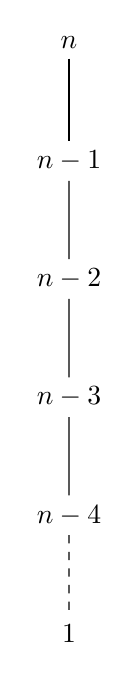
\begin{tikzpicture}
\node{$n$}
    child{node{$n - 1$}
        child{node{$n - 2$}
            child{node{$n - 3$}
                child{node{$n - 4$}
                    child{node{1}
                            edge from parent [dashed]
                    }
                }  
            }
        }
    };
\end{tikzpicture}
\end{center}
\[\text{height} = n - 1\]
\[\text{at depth $i$, cost = (number of nodes)(cost per node)} = (1)(n - i) = n - i\]
\[\text{number of leaves} = 1\]
\begin{align*}
    T(n) &=\sum_{i = 0}^{n - 1} (n - i)\\
    &= \sum_{i = 0}^{n - 1} n - \sum_{i = 0}^{n - 1} i\\
    &\text{/* since} \sum_{i = 0}^{n} i = \frac{n(n + 1)}{2} \text{ */}\\
    &= n^2 - \frac{(n - 1)((n - 1) + 1)}{2}\\
    &= n^2 - \frac{(n - 1)n}{2}\\
    &= n^2 - \frac{n^2 - n}{2}\\
    &= \frac{2n^2}{2} - \frac{n^2 - n}{2}\\
    &= \frac{2n^2 - n^2 + n}{2}\\
    &= \frac{n^2 + n}{2}\\
    &= \frac{1}{2}n^2 + \frac{1}{2}n\\
    &= \Theta(n^2)\\
\end{align*}
\newpage
\noindent
(b)
\[T(n) = 2T(n/4) + \sqrt{n}\]
\begin{center}
\begin{tikzpicture}
[
    level 1/.style = {sibling distance = 6cm, level distance = 2cm},
    level 2/.style = {sibling distance = 3cm, level distance = 2cm},
    level 3/.style = {sibling distance = 1.5cm, level distance = 2cm},
]
    \node{$\sqrt{n}$}
        child{node{$\sqrt{n / 4^1}$}
            child{node{$\sqrt{n / 4^2}$}
                child{node{$\sqrt{n / 4^3}$}
                    child{node{1\;$\cdots$}
                    edge from parent [dashed]
                    }
                    child{node{$\cdots$}
                    edge from parent [dashed]
                    }
                }
                child{node{$\sqrt{n / 4^3}$}
                    child{node{$\cdots$}
                    edge from parent [dashed]
                    }
                    child{node{$\cdots$}
                    edge from parent [dashed]
                    }
                }
            }
            child{node{$\sqrt{n / 4^2}$}
                child{node{$\sqrt{n / 4^3}$}
                    child{node{$\cdots$}
                    edge from parent [dashed]
                    }
                    child{node{$\cdots$}
                    edge from parent [dashed]
                    }
                }
                child{node{$\sqrt{n / 4^3}$}
                    child{node{$\cdots$}
                    edge from parent [dashed]
                    }
                    child{node{$\cdots$}
                    edge from parent [dashed]
                    }
                }
            }
        }
        child{node{$\sqrt{n / 4^1}$}
            child{node{$\sqrt{n / 4^2}$}
                child{node{$\sqrt{n / 4^3}$}
                    child{node{$\cdots$}
                    edge from parent [dashed]
                    }
                    child{node{$\cdots$}
                    edge from parent [dashed]
                    }
                }
                child{node{$\sqrt{n / 4^3}$}
                    child{node{$\cdots$}
                    edge from parent [dashed]
                    }
                    child{node{$\cdots$}
                    edge from parent [dashed]
                    }
                }
            }
            child{node{$\sqrt{n / 4^2}$}
                child{node{$\sqrt{n / 4^3}$}
                    child{node{$\cdots$}
                    edge from parent [dashed]
                    }
                    child{node{$\cdots$}
                    edge from parent [dashed]
                    }
                }
                child{node{$\sqrt{n / 4^3}$}
                    child{node{$\cdots$}
                    edge from parent [dashed]
                    }
                    child{node{$\cdots$\;1}
                    edge from parent [dashed]
                    }
                }
            }
        };
\end{tikzpicture}    
\end{center}
\[n / 4^i = 1, \qquad n = 4^i, \qquad \log_4 n = i\]
\[\text{height} = \log_4 n\]
\begin{align*}
\text{at depth } i , \text{cost} &= \text{(number of nodes)(cost per node)} = (2^i)\sqrt{\left(\frac{n}{4^i}\right)}\\
&= (2^i)\left(\frac{\sqrt{n}}{2^i}\right)\\
&= \sqrt{n}\\
\end{align*}
\[\text{number of leaves} = 2^{\log_4 n} = n^{\log_4 2} = n^{1 / 2}\]
/* since $\log_4(\textcolor{orchid}{2^{\log_4 n}}) = (\log_4 n)(\log_4 2) = (\log_4 2)(\log_4 n) = \log_4 (\textcolor{orchid}{n^{\log_4 2}})$ */
\begin{align*}
    T(n) &= \sum_{i = 0}^{\log_4 n - 1} \sqrt{n} + \Theta(n^{1/ 2})\\
    &= (\log_4 n - 1 + 1) \sqrt{n} + \Theta(n^{1/ 2})\\
    &= \sqrt{n}\log_4 n + \Theta(n^{1/ 2})\\
    &= \Theta(\sqrt{n}\log_4 n)\\
\end{align*}
\newpage
\noindent
(c)
\[T(n) = 9T(n/3) + n^2\]
\begin{center}
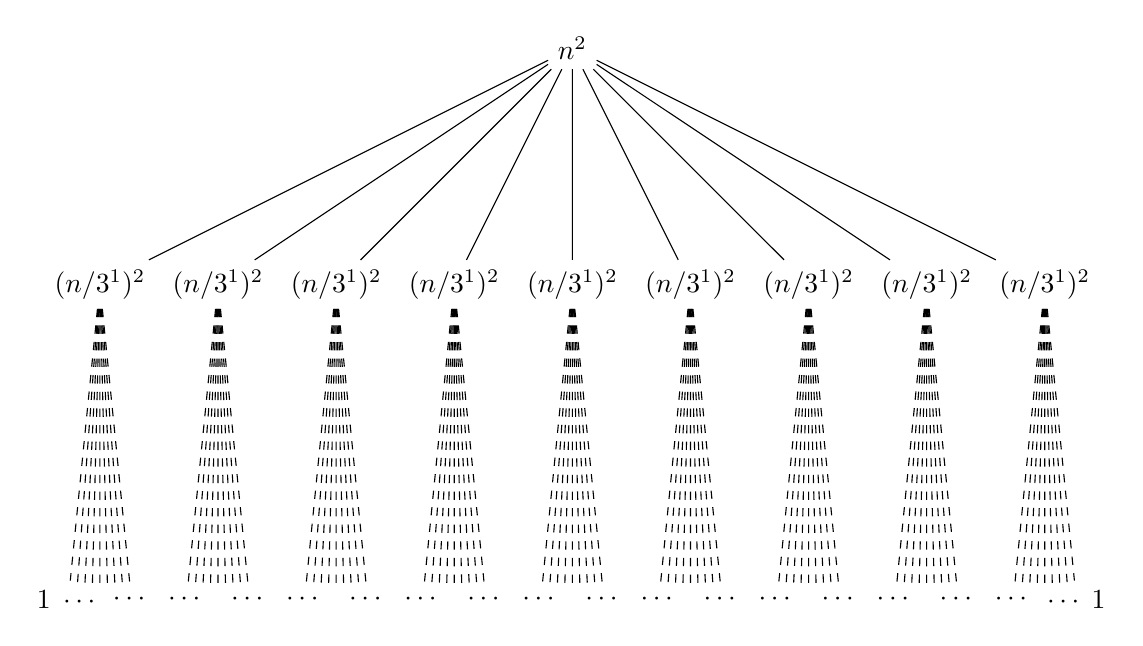
\begin{tikzpicture}
[
    level 1/.style = {sibling distance = 1.5cm, level distance = 3cm},
    level 2/.style = {sibling distance = 0.1cm, level distance = 4cm},
]
\node{$n^2$}
    child{node{$(n / 3^1)^2$}
        child{node{$1\;\cdots$} edge from parent[dashed]}
        child{node{} edge from parent[dashed]}
        child{node{} edge from parent[dashed]}
        child{node{} edge from parent[dashed]}
        child{node{} edge from parent[dashed]}
        child{node{} edge from parent[dashed]}
        child{node{} edge from parent[dashed]}
        child{node{} edge from parent[dashed]}
        child{node{$\cdots$} edge from parent[dashed]}
    }
    child{node{$(n / 3^1)^2$}
        child{node{$\cdots$} edge from parent[dashed]}
        child{node{} edge from parent[dashed]}
        child{node{} edge from parent[dashed]}
        child{node{} edge from parent[dashed]}
        child{node{} edge from parent[dashed]}
        child{node{} edge from parent[dashed]}
        child{node{} edge from parent[dashed]}
        child{node{} edge from parent[dashed]}
        child{node{$\cdots$} edge from parent[dashed]}
    }
    child{node{$(n / 3^1)^2$}
        child{node{$\cdots$} edge from parent[dashed]}
        child{node{} edge from parent[dashed]}
        child{node{} edge from parent[dashed]}
        child{node{} edge from parent[dashed]}
        child{node{} edge from parent[dashed]}
        child{node{} edge from parent[dashed]}
        child{node{} edge from parent[dashed]}
        child{node{} edge from parent[dashed]}
        child{node{$\cdots$} edge from parent[dashed]}
    }
    child{node{$(n / 3^1)^2$}
        child{node{$\cdots$} edge from parent[dashed]}
        child{node{} edge from parent[dashed]}
        child{node{} edge from parent[dashed]}
        child{node{} edge from parent[dashed]}
        child{node{} edge from parent[dashed]}
        child{node{} edge from parent[dashed]}
        child{node{} edge from parent[dashed]}
        child{node{} edge from parent[dashed]}
        child{node{$\cdots$} edge from parent[dashed]}
    }
    child{node{$(n / 3^1)^2$}
        child{node{$\cdots$} edge from parent[dashed]}
        child{node{} edge from parent[dashed]}
        child{node{} edge from parent[dashed]}
        child{node{} edge from parent[dashed]}
        child{node{} edge from parent[dashed]}
        child{node{} edge from parent[dashed]}
        child{node{} edge from parent[dashed]}
        child{node{} edge from parent[dashed]}
        child{node{$\cdots$} edge from parent[dashed]}
    }
    child{node{$(n / 3^1)^2$}
        child{node{$\cdots$} edge from parent[dashed]}
        child{node{} edge from parent[dashed]}
        child{node{} edge from parent[dashed]}
        child{node{} edge from parent[dashed]}
        child{node{} edge from parent[dashed]}
        child{node{} edge from parent[dashed]}
        child{node{} edge from parent[dashed]}
        child{node{} edge from parent[dashed]}
        child{node{$\cdots$} edge from parent[dashed]}
    }
    child{node{$(n / 3^1)^2$}
        child{node{$\cdots$} edge from parent[dashed]}
        child{node{} edge from parent[dashed]}
        child{node{} edge from parent[dashed]}
        child{node{} edge from parent[dashed]}
        child{node{} edge from parent[dashed]}
        child{node{} edge from parent[dashed]}
        child{node{} edge from parent[dashed]}
        child{node{} edge from parent[dashed]}
        child{node{$\cdots$} edge from parent[dashed]}
    }
    child{node{$(n / 3^1)^2$}
        child{node{$\cdots$} edge from parent[dashed]}
        child{node{} edge from parent[dashed]}
        child{node{} edge from parent[dashed]}
        child{node{} edge from parent[dashed]}
        child{node{} edge from parent[dashed]}
        child{node{} edge from parent[dashed]}
        child{node{} edge from parent[dashed]}
        child{node{} edge from parent[dashed]}
        child{node{$\cdots$} edge from parent[dashed]}
    }
    child{node{$(n / 3^1)^2$}
        child{node{$\cdots$} edge from parent[dashed]}
        child{node{} edge from parent[dashed]}
        child{node{} edge from parent[dashed]}
        child{node{} edge from parent[dashed]}
        child{node{} edge from parent[dashed]}
        child{node{} edge from parent[dashed]}
        child{node{} edge from parent[dashed]}
        child{node{} edge from parent[dashed]}
        child{node{$\cdots\;1$} edge from parent[dashed]}
    };
\end{tikzpicture}    
\end{center}
\[n / 3^i = 1, \qquad n = 3^i, \qquad \log_3 n = i\]
\[\text{height} = \log_3 n\]
\begin{align*}
    \text{at depth } i , \text{cost} &= \text{(number of nodes)(cost per node)} \\
    &= (9^i)\left(\frac{n}{3^i}\right)^2\\
    &= (n^2)\left(\frac{9^i}{9^i}\right) = n^2\\
\end{align*}
\[\text{number of leaves} = 9^{\log_3 n} = n^{\log_3 9} = n^2\]
/* since $\log_3(\textcolor{orchid}{9^{\log_3 n}}) = (\log_3 n)(\log_3 9) = (\log_3 9)(\log_3 n) = \log_3 (\textcolor{orchid}{n^{\log_3 9}})$ */
\begin{align*}
    T(n) &= \sum_{i = 0}^{\log_3 n - 1} n^2 + \Theta(n^2)\\
    &= (\log_3 n - 1 + 1) n^2 + \Theta(n^2)\\
    &= n^2\log_3 n + \Theta(n^2)\\
    &= \Theta(n^2\log_3 n)\\
\end{align*}
\newpage
\noindent
(d)
\[T(n) = T(n / 2) + 1\]
for a recurrence $T(n) = aT(n / b) + f(n)$, draw an $a$-ary tree, here $a = 1$, so draw a 1-ary tree:\\
\begin{center}
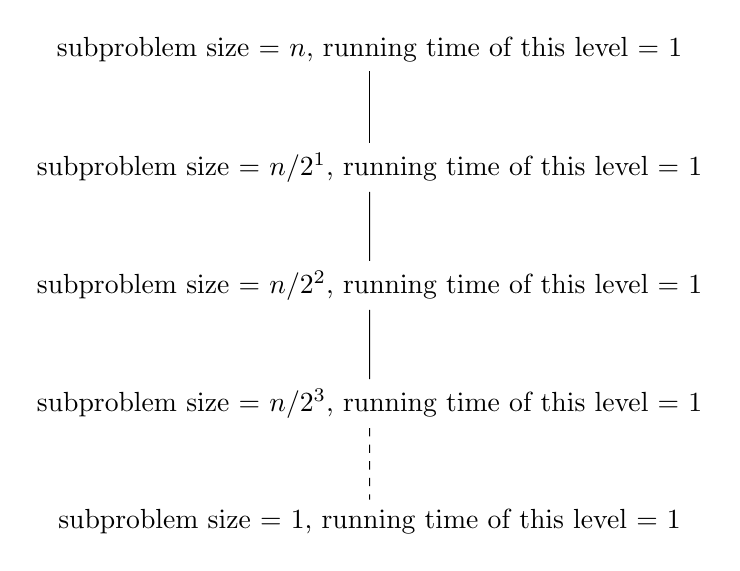
\begin{tikzpicture}
    \node{subproblem size = $n$, running time of this level = 1}
        child{node{subproblem size = $n / 2^1$, running time of this level = 1}
           child{node{subproblem size = $n / 2^2$, running time of this level = 1}
                child{node{subproblem size = $n / 2^3$, running time of this level = 1}
                    child{node{subproblem size = 1, running time of this level = 1} edge from parent [dashed]}
                }
           }
        };
\end{tikzpicture}
\end{center}
\\
\[n / 2^i = 1, \qquad n = 2^i, \qquad \log_2 n = i\]
\[\text{height} = \log_2 n\]
\begin{align*}
     \text{at depth } i , \text{cost} &= \text{(number of nodes)(cost per node)}\\
     &= (1)(1)\\
     &= 1\\
\end{align*}
\[\text{number of leaves} = 1\]
\begin{align*}
    T(n) &= \sum_{i = 0}^{\log_2 n - 1} 1 + \Theta(1)\\
    &= (\log_2 n - 1 + 1)(1) + \Theta(1)\\
    &= \log_2 n + \Theta(1)\\
    &= \Theta(\log_2 n)\\
\end{align*}
\newpage
\noindent
Problem 4
\begin{lstlisting}[language = c, mathescape = true, escapeinside = {(*}{*)}]
MERGE($A,\; p,\; q,\; r$)
1   $n_1 = q - p + 1$
2   $n_2 = r - q$
3   let $L[1...n_1 + 1]$ and $R[1...n_2 + 1]$ be new arrays
4   for $i = 1$ (*\textbf{to}*) $n_1$
5       $L[i] = A[p + i - 1]$
6   for $j = 1$ (*\textbf{to}*) $n_2$
7       $R[j] = A[q + j]$
8   $L[n_1 + 1] = \infty$
9   $R[n_2 + 1] = \infty$
10  $i = 1$
11  $j = 1$
12  for $k = p$ (*\textbf{to}*) $r$
13      if $L[i] \leq R[j]$
14           $A[k] = L[i]$
15           $i = i + 1$
16      else $A[k] = R[j]$
17           $j = j + 1$


MERGE_SORT($A,\;p,\;r$)
1 if $p < r$
2   $q = p + \lfloor (r - p) / 2 \rfloor$
3   MERGE_SORT($A,\; p,\; q$)
4   MERGE_SORT($A,\; q + 1,\; r$)
5   MERGE($A,\; p,\; q,\; r$)
\end{lstlisting}
\\
a sorting algorithm is stable if elements with the same key maintain their relative ordering in the output array as their relative ordering in the input array\\
\\
preserve relative ordering means that if element $a$ and element $b$ have equal keys, and if element $a$'s index is smaller than element $b$'s index in the input array, then $a$'s index must also be smaller than $b$'s index in the output array. $\forall (i,\; j) \in \{[1, A.length] \cap \mathbb{N}\}^2$, if element $a$ is stored in $A[i]$ in the input array and element $b$ is stored in $A[j]$ in the input array, and if $i < j$ and $A[i].key = A[j].key$, then $a$ and $b$'s final positions $i'$ and $j'$ in the output array of MERGE\_SORT must satisfy $i' < j'$\\
\\
loop invariant: at the start of the each \textbf{for} iteration in line 12 of MERGE(), elements with the same key in $A[p...k - 1]$ preserve their relative ordering\\
\\
initialization: before first iteration of the loop, $k = p$, so subarray $A[p...k - 1]$ is empty. so loop invariant is true\\
\\
maintenance: MERGE\_SORT is stable because of the comparison in line 13 of MERGE(), if two elements $L[i]$ and $R[j]$ are equal, the element $L[i]$ in the left subarray $L$ will be put first into the merged array $A$ without changing the original relative ordering (since $L[i]$ comes from the left subarray, $L[i]$ comes before $R[j]$ in the input array, and since $L[i]$ is put first into the merged array $A$ before $R[j]$ is put into the merged array $A$, $L[i]$ will come before $R[j]$ in the output array). incrementing $k$ (in the \textbf{for} loop update) and incrementing $i$ (in line 15) reestablishes the loop invariant for the next iteration\\
\\
termination: at termination, $k = r + 1$. by the loop invariant, all of the elements with the same key in the subarray $A[p...k - 1]$ preserve their relative ordering\\
\newpage 
\noindent
Problem 5
\begin{lstlisting}[mathescape = true, language = c]
/* find() is a divide-and-conquer algorithm that finds
the largest number among the elements of A */

max(m1, m2)
{
    if(m1 >= m2)
        return m1;
    else
        return m2;
}

find_max(A, int L, int h, max)
{
    if(L >= h)
        return max;
    int mid = L + $\lfloor$ (h - L) / 2 $\rfloor$;
    if(A[mid] > max)
        max = A[mid];
    m1 = find_max(A, L, mid, max);
    m2 = find_max(A, mid + 1, h, max);
    return max(m1, m2);
}

find(A)
{
    return find_max(A, 1, A.length, $-\infty$));
}
\end{lstlisting}
\end{document}